In graph theory, the clique -- also called complete graph -- is a set of nodes such that each node is adjacent to all others. This is expressed in the present context by a set called \textit{macrocolonne} consisting of neurons or group of neurons called \textit{microcolonne} interconnected according to the type of information concerned -- see figures \ref{fig:cli}(a), \ref{fig:cli}(b) and \ref{fig:cli}(c).

\begin{figure}[htbp]
\begin{center}
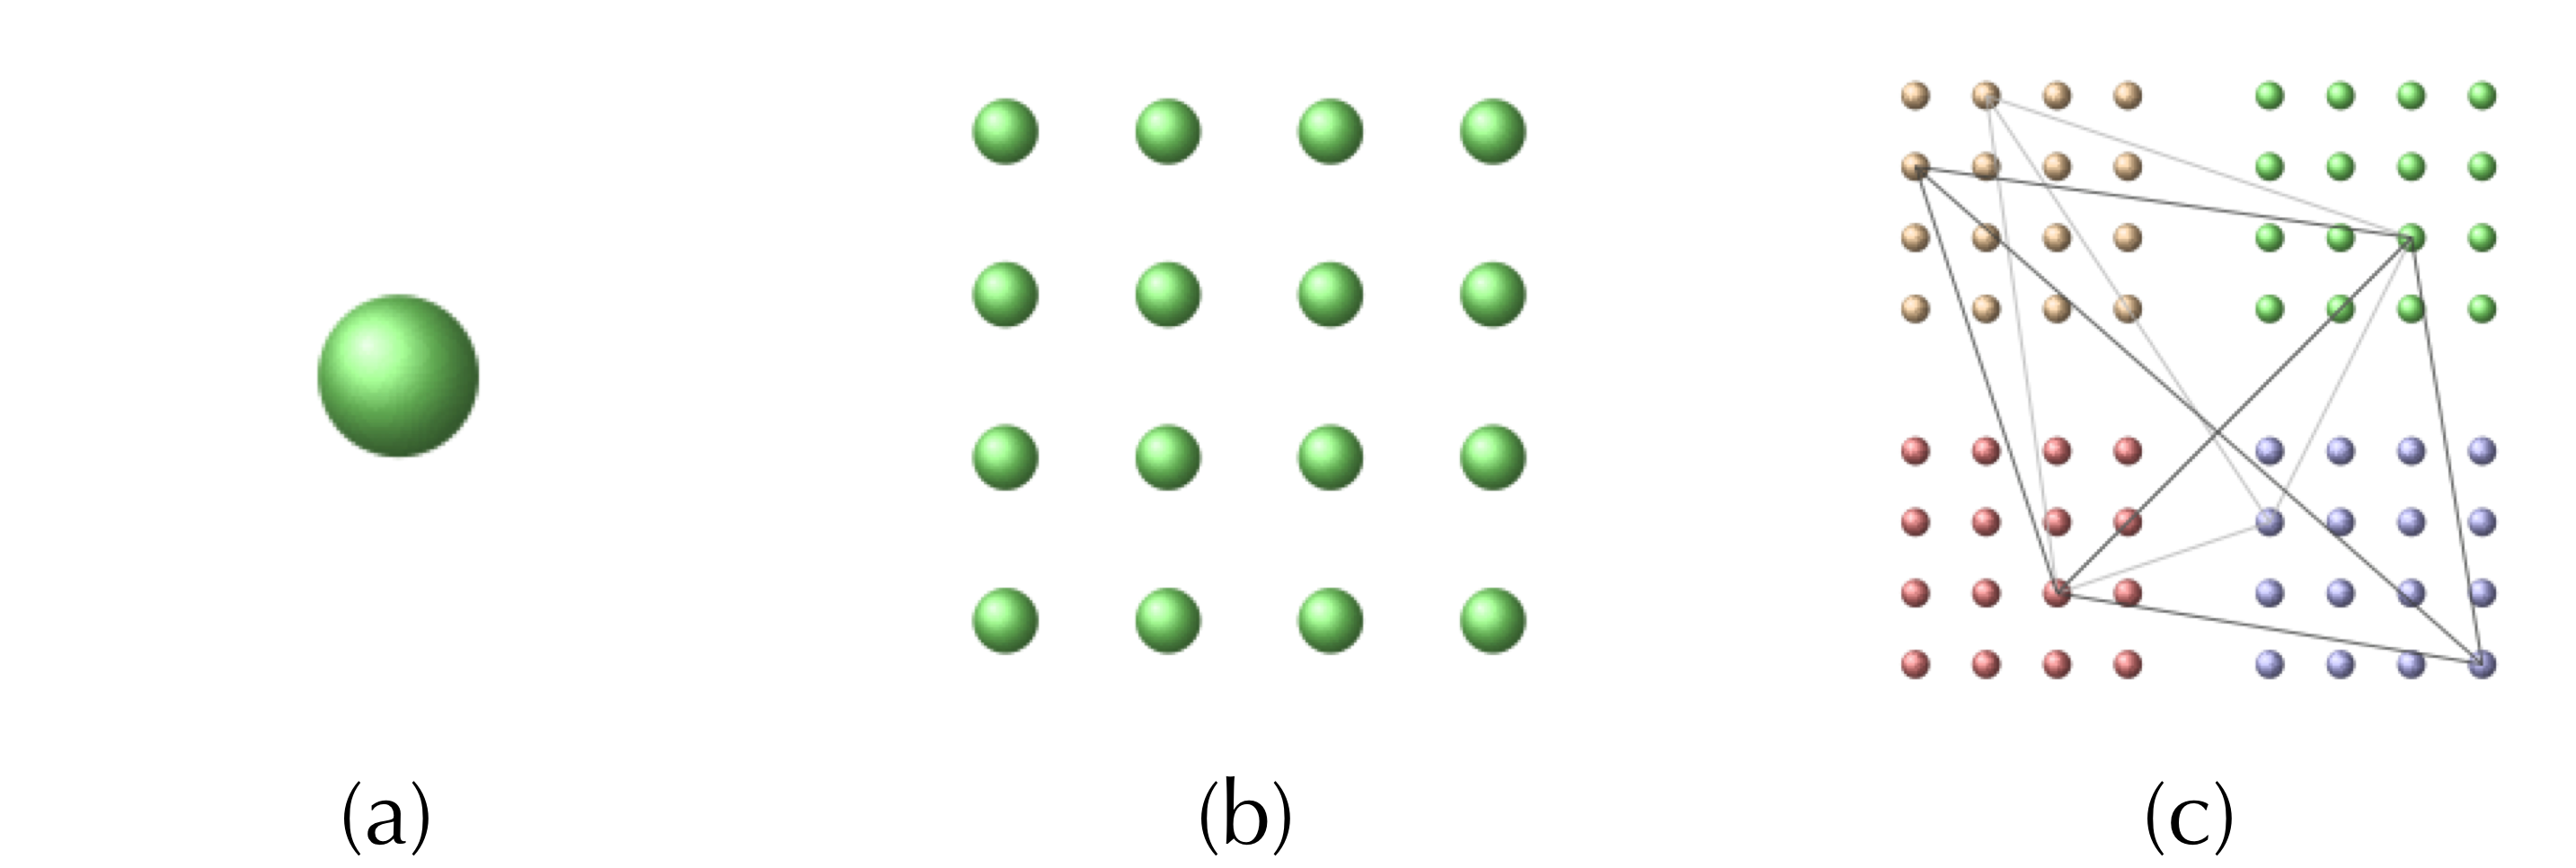
\includegraphics[width=\columnwidth]{2501}
\caption{(a) \textit{Microcolonne}: neuron or group of neurons carrying information in terms of activation potential -- e.g. a pitch of a sound. (b) \textit{Colonne}: region of \textit{microcolonnes} carrying the same type of information -- e.g. a set of pitches as a scale or other. (c) \textit{Macrocolonne}: a region of \textit{colonnes} able to carry `complete' information called `\textit{infon}' as a clique -- e.g. the characteristics of a sound defined by its pitch, intensity, duration and timbre.}
\label{fig:cli}
\end{center}
\end{figure}

On the figure \ref{fig:cli}(c), we can observe two cliques, one of which is dark gray overlays partially on the second in light gray.

\bigskip

From now on, we name indifferently as synonym \textit{microcolonnes} as \textit{fanaux} (i.e. a list of NEURON),  \textit{colonne} as MLT, \textit{macrocolonne} as AREA and \textit{infon} as a clique at the AREA level.